\documentclass{article}
\usepackage[spanish, es-tabla]{babel}
\usepackage[utf8]{inputenc}
\usepackage[colorlinks=true]{hyperref}
\usepackage{minted}
\usepackage{amsmath}
\usepackage{geometry}
\usepackage{graphicx}
\usepackage{tabularx}
\usepackage{array}
\usepackage{colortbl}
\usepackage{booktabs}
\usepackage{multirow}
\usepackage{subcaption}
\usepackage{wrapfig}
\usepackage{tabu}
\usepackage{blindtext}
\usepackage[table]{xcolor}
\usepackage[style=ieee]{biblatex}


\setlength{\arrayrulewidth}{0.5mm}
\setlength{\tabcolsep}{12pt}
\renewcommand{\arraystretch}{1}
\addbibresource{references.bib}
\newcolumntype{s}{>{\columncolor{green}} l}
\geometry{verbose,tmargin=3cm,bmargin=3cm,lmargin=3cm,rmargin=6.8cm}
% \newcolumntype{Y}{>{\centering\arraybackslash}X}
\definecolor{algo}{RGB}{170, 170, 255}

\newenvironment{exampletwoup}
  {\VerbatimEnvironment
   \begin{VerbatimOut}{example.out}}
  {\end{VerbatimOut}
   \setlength{\parindent}{0pt}
   \fbox{\begin{tabular}{l|l}
   \begin{minipage}{0.55\linewidth}
     \inputminted[fontsize=\small,resetmargins]{latex}{example.out}
   \end{minipage} &
   \begin{minipage}{0.35\linewidth}
     \input{example.out}
   \end{minipage}
\end{tabular}}}


\begin{document}
\begin{minted}[frame=single]{bibtex}
@article{einstein,
  author = "Albert Einstein",
  title = "{Zur Elektrodynamik bewegter K{\"o}rper}. ({German})
  [{On} the electrodynamics of moving bodies]",
  journal = "Annalen der Physik",
  volume = "322",
  number = "10",
  pages = "891--921",
  year = "1905",
  DOI = "http://dx.doi.org/10.1002/andp.19053221004",
  keywords = "physics"
}
\end{minted}
% El artículo de Einstein \cite{einstein} y el 
% libro de Dirac \cite{dirac} están relacionados con la física.

% \printbibliography

% \begin{minted}[frame=single]{latex}
% \usepackage{adjustbox}
% \begin{adjustbox}{max width=...}
%   % tabular...
% \end{adjustbox}
% \end{minted}
% Cambiando el color del texto, \textbf{\textcolor{red}{rojo}}, \textcolor[RGB]{0, 255, 0}{verde}, y \textcolor{blue}{azul}. \\ \\
% \arrayrulecolor[RGB]{123, 145, 255}
% \begin{tabular}{|s|l|l|l|} \hline
%   \rowcolor{orange} Item 1 & item 2 & item 3 & \cellcolor[HTML]{8A4B08}item 4 \\
%   Item 5 & item 6 & item 7 & item 8 \\
%   \arrayrulecolor{black}
%   Item 9 & \cellcolor{red}item 10 & item 11 & item 12 \\ \cline{2-3}
%   \arrayrulecolor[RGB]{230, 200, 100}
%   Item 13 & item 14 & item 15 & item 16 \\ \hline
% \end{tabular} \\ \\

% \arrayrulecolor{black}
% {\rowcolors{1}{algo}{red}
% \begin{tabular}{|l|l|l|l|} \hline
%   Item 1 & item 2 & item 3 & item 4 \\ \hline
%   Item 5 & item 6 & item 7 & item 8 \\ \hline
%   Item 9 & item 10 & item 11 & item 12 \\ \hline
%   Item 13 & item 14 & item 15 & item 16 \\ \hline
% \end{tabular}}
% \begin{minted}[frame=single]{latex}
% % Preámbulo
% \setlength{\arrayrulewidth}{1mm}
% \setlength{\tabcolsep}{18pt}
% \renewcommand{\arraystretch}{1.5}
% \end{minted}
% \begin{tabular}{ |p{3cm}|p{3cm}|p{3cm}|  }
%   \hline
%   \multicolumn{3}{|c|}{Country List} \\
%   \hline
%   Country Name     or Area Name& ISO ALPHA 2 Code &ISO ALPHA 3 \\
%   \hline
%   Afghanistan & AF &AFG \\
%   Aland Islands & AX   & ALA \\
%   Albania &AL & ALB \\
%   Algeria    &DZ & DZA \\
%   American Samoa & AS & ASM \\
%   Andorra & AD & AND   \\
%   Angola & AO & AGO \\
%   \hline
% \end{tabular}
% \begin{minted}[frame=single]{latex}
% Por aquí viene el texto...

% \begin{wraptable}{aligment}{width}
%   \centering
%   \begin{tabular}{columnas}
%     % contenido de la tabla
%   \end{tabular}
%   \caption{Descripción}
%   \label{tab:etiqueta}
% \end{wraptable}

% Y por aquí sigue el texto, rodeando la tabla...
% \end{minted}

% \blindtext

% \begin{wraptable}{r}{0.5\textwidth}
%   \centering
%   \begin{tabular}{||l|l||} \hline
%     algo & algo \\
%     algo & algo \\ \hline
%   \end{tabular}
%   \caption{Descripción}
%   \label{tab:etiqueta}
% \end{wraptable}

% \blindtext

% \begin{tabular}{|s|m{3cm}|m{3cm}|} \hline
% En esta celda hay mucho texto, pero se acomoda porque la longitud de la columna es fija & celda 2 & celda 3 \\ \hline
% En esta celda sucede lo mismo & celda 5 & celda 6 \\ \hline
% celda 7 & celda 8 & celda 9 \\ \hline
% \end{tabular}

% \begin{minted}[frame=single]{latex}
% \begin{tabular}{|m{5em}|m{1cm}|m{1cm}|} \hline
%   texto & celda 2 & celda 3 \\ \hline
%   más texto & celda 5 & celda 6 \\ \hline
%   celda 7 & celda 8 & celda 9 \\ \hline
% \end{tabular}
% \end{minted}}

% \begin{minted}[frame=single]{latex}
%   \begin{tabu} to 0.5\textwidth {|X[l]|X[c]|X[r]|}\hline
%     item 11  & item 12 & item 13 \\ \hline
%     item 21  & item 22  & item 23 \\ \hline
%   \end{tabu}
% \end{minted}
  
% \begin{minted}[frame=single]{latex}
%   Por aquí viene el texto...

%   \begin{wrapfigure}{aligment}{width}
%     \includegraphics[options]{figname}
%     \caption{Descripción}
%     \label{fig:etiqueta}
%   \end{wrapfigure}
  
%   Por acá sigue el texto, rodeando la imagen...
% \end{minted}

% \begin{wrapfigure}{l}{0.25\textwidth}
%   \centering
%   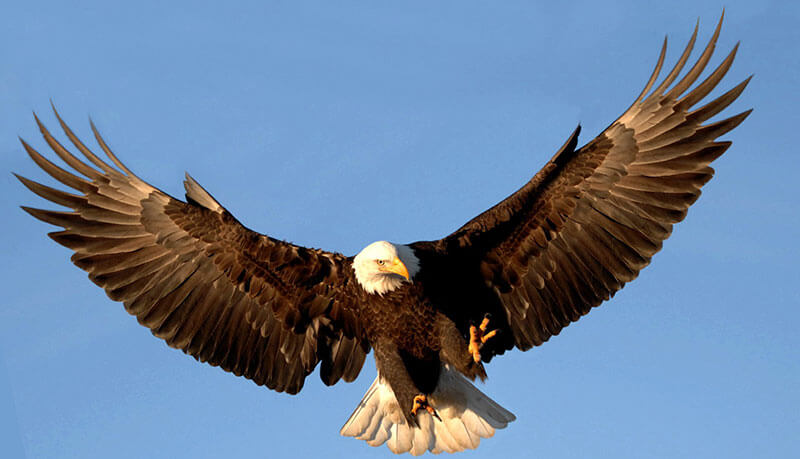
\includegraphics[width=0.9\linewidth]{aguila}
%   \caption{Águila}
%   \label{fig:aguila}
% \end{wrapfigure}


% \begin{tabular}{||c|l||} \hline
%   \emph{Parámetro} & \emph{Posición} \\ \hline
%   \texttt{h} & \emph{aquí} si es posible\\
%   \texttt{t} & al \emph{inicio} de la página \\
%   \texttt{b} & al \emph{final} de la página \\
%   \texttt{p} & en una \emph{página} especial de solo flotantes \\
%   \texttt{!} & ignorar aspectos estéticos \\
%   \texttt{H} & \emph{aquí} definitivamente. Se requiere el paquete \emph{float} \\ \hline
% \end{tabular}

% \begin{tabular}{||l|l||} \hline
%   \emph{Abreviación} & \emph{Definición} \\ \hline
%   \verb|pt| & un punto, es la unidad por defecto. Alrededor de 0.3515 mm \\
%   \verb|mm| & un milímetro \\
%   \verb|cm| & un centímetro \\
%   \verb|in| & una pulgada \\
%   \verb|ex| & el alto de una \textbf{x} en la fuente actual \\
%   \verb|em| & el ancho de una \textbf{m} en la fuente actual \\
%   \verb|\columnsep| & distancia entre columnas \\
%   \verb|\columnwidth| & ancho de la columna \\
%   \verb|\linewidth| & ancho de la línea en el ambiente actual \\
%   \verb|\paperwidth| & ancho de la página \\
%   \verb|\paperheight| & alto de la página \\
%   \verb|\textwidth| & ancho del texto \\
%   \verb|\textheight| & alto del texto \\
%   \verb|\unitlenght| & unidades de logitud en el ambiente \emph{picture} \\ \hline
% \end{tabular}

% \begin{tabular}{||l|l||l|l||l|l||} \hline
%   \emph{declaración} & \emph{tamaño} & \emph{declaración} & \emph{tamaño} & \emph{declaración} & \emph{tamaño} \\ \hline
%   \texttt{\{\textbackslash tiny ...\}} & \tiny size & \texttt{\{\textbackslash normalsize ...\}} & \normalsize size & & \\
%   \texttt{\{\textbackslash scriptsize ...\}} & \scriptsize size & \texttt{\{\textbackslash large ...\}} & \large size & & \\
%   \texttt{\{\textbackslash footnotesize ...\}} & \footnotesize size & \texttt{\{\textbackslash Large ...\}} & \Large size & \texttt{\{\textbackslash huge ...\}} & \huge size\\
%   \texttt{\{\textbackslash small ...\}} & \small size & \texttt{\{\textbackslash LARGE ...\}} & \LARGE size & \texttt{\{\textbackslash Huge ...\}} & \Huge size \\ \hline
% \end{tabular}


% Test 
% \begin{table}
%   \centering
% 	\begin{subtable}[b]{0.45\textwidth}
% 		\centering
% 		\resizebox{0.9\textwidth}{!}{\begin{tabular}{|c|c|c|c|c|} \hline
% 			       & \multicolumn{4}{c|}{Calificaciones}                                      \\ \hline
% 			Nombre & Parcial 1                           & Parcial 2 & Parcial 3 & Definitiva \\ \hline
% 			Pedro  & 4.5                                 & 4.6       & 4.8       & 4.6        \\
% 			Alicia & 5.0                                 & 4.8       & 5.0       & 4.9        \\
% 			Johana & 3.4                                 & 2.8       & 2.9       & 3.0        \\ \hline
% 		\end{tabular}}
% 		% \caption{\label{tab:notas} Estas son las notas de Física: Mecánica}
% 		\caption{Tabla a}
%   \end{subtable}%
% 	\begin{subtable}[b]{0.45\textwidth}
% 		\centering
% 		\resizebox{0.9\textwidth}{!}{\begin{tabular}{|c|c|c|c|c|} \hline
% 			       & \multicolumn{4}{c|}{Calificaciones}                                      \\ \hline
% 			Nombre & Parcial 1                           & Parcial 2 & Parcial 3 & Definitiva \\ \hline
% 			Pedro  & 4.5                                 & 4.6       & 4.8       & 4.6        \\
% 			Alicia & 5.0                                 & 4.8       & 5.0       & 4.9        \\
% 			Johana & 3.4                                 & 2.8       & 2.9       & 3.0        \\ \hline
% 		\end{tabular}}
% 		% \caption{\label{tab:notas} Estas son las notas de Física: Mecánica}
% 		\caption{Tabla b}
% 	\end{subtable}
% 	\caption{Dos subtablas}
% \end{table}

% Test
% La figura \ref{fig:animales} muestra varios animales.
% \begin{figure}[h!]
%   \centering
%   \begin{subfigure}[b]{0.3\textwidth}
%     \centering
%     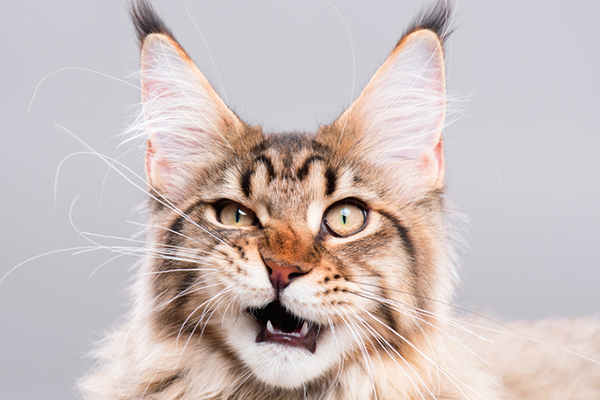
\includegraphics[width=0.9\linewidth, height=0.6\linewidth]{gato}
%     \caption{Gato}\label{fig:gato}
%   \end{subfigure}
%   \begin{subfigure}[b]{0.3\textwidth}
%     \centering
%     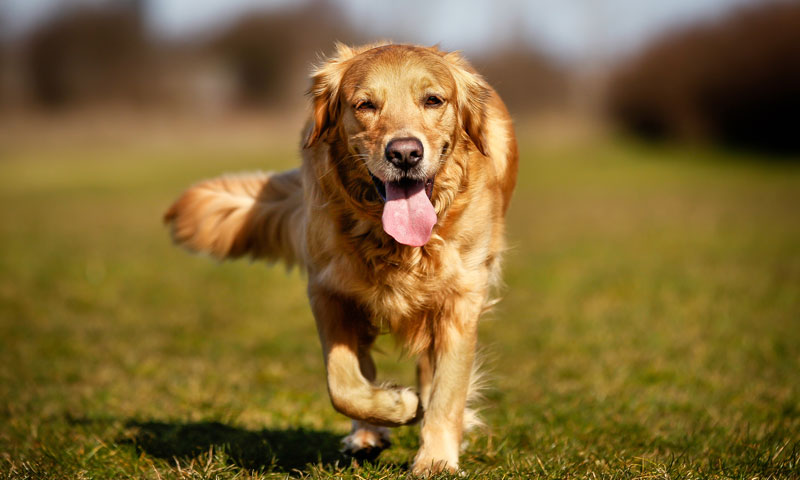
\includegraphics[width=0.9\linewidth, height=0.6\linewidth]{perro}
%     \caption{Perro}\label{fig:perro}
%   \end{subfigure}
%   \begin{subfigure}[b]{0.3\textwidth}
%     \centering
%     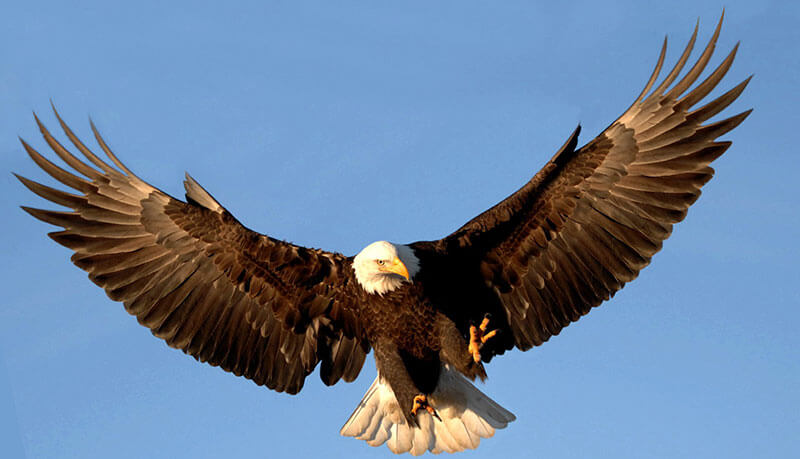
\includegraphics[width=0.9\linewidth, height=0.6\linewidth]{aguila}
%     \caption{Águila}\label{fig:aguila}
%   \end{subfigure}
%   \caption{Algunos animales}\label{fig:animales}
% \end{figure}


\end{document}